\begin{IEEEbiography}
[{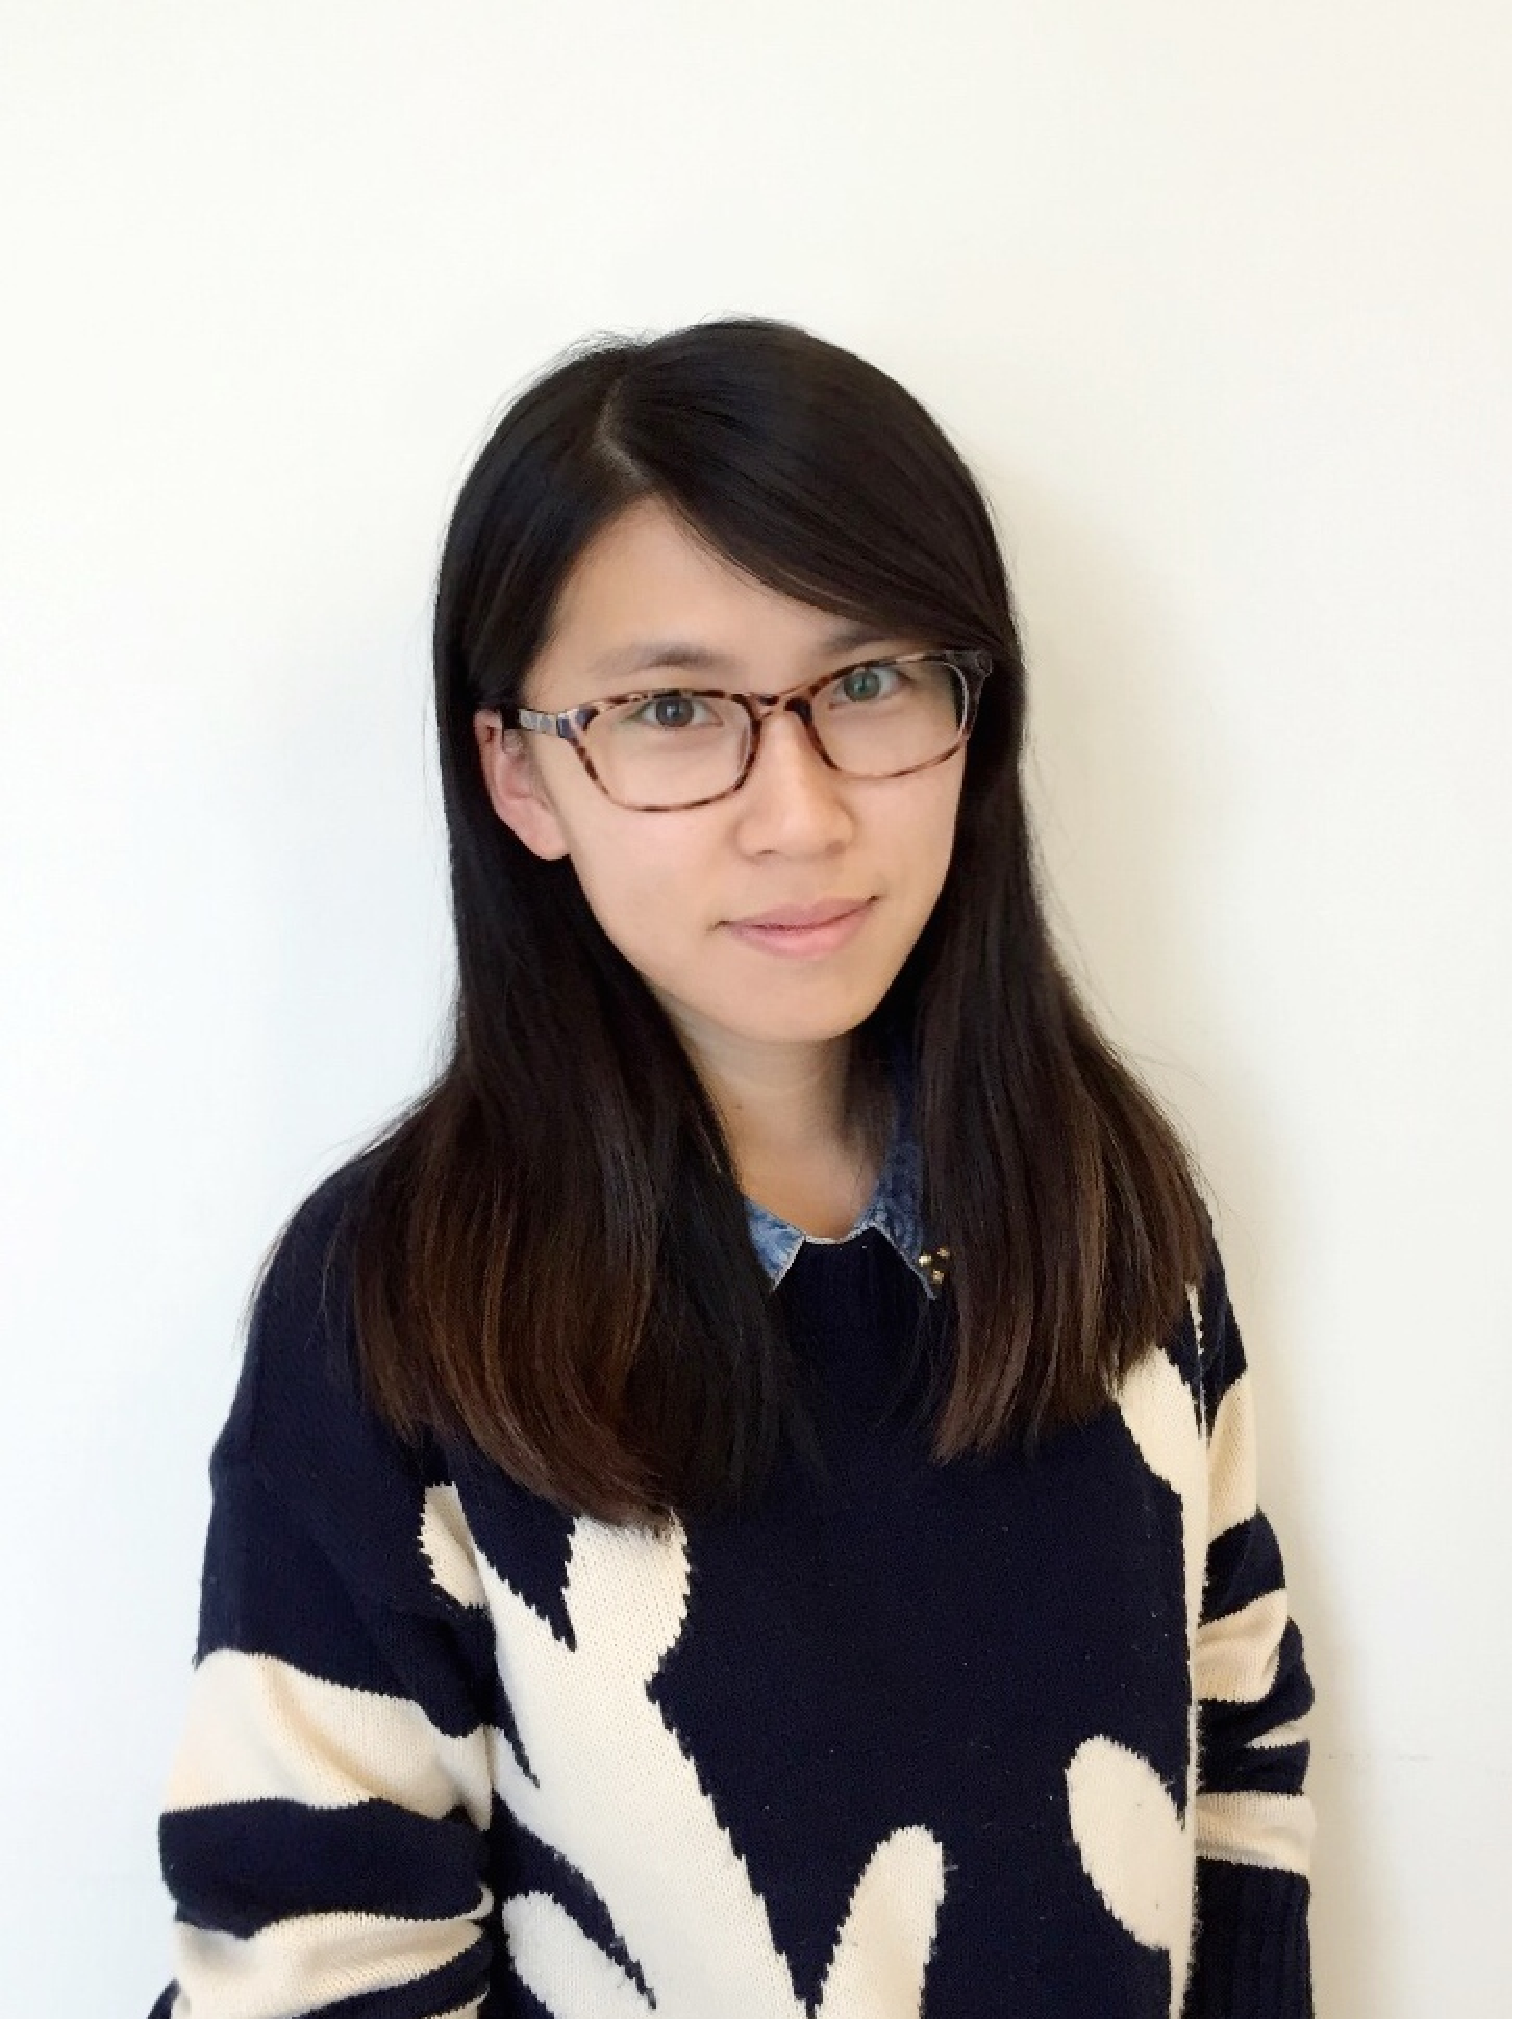
\includegraphics[width=1in,height=1.25in,clip,keepaspectratio]{Liu.pdf}}]
{Menghan Liu} received the B.E. degree in communication engineering from Tianjin University, Tianjin, China. She is currently pursuing the M.S. degree with the Electrical Engineering and Computer Science Department at Case Western Reserve University. Her research interests lie in the area of image processing, computer vision, augmented reality, big data analysis, wearable computing and personal health.
\end{IEEEbiography}
\begin{IEEEbiography}
[{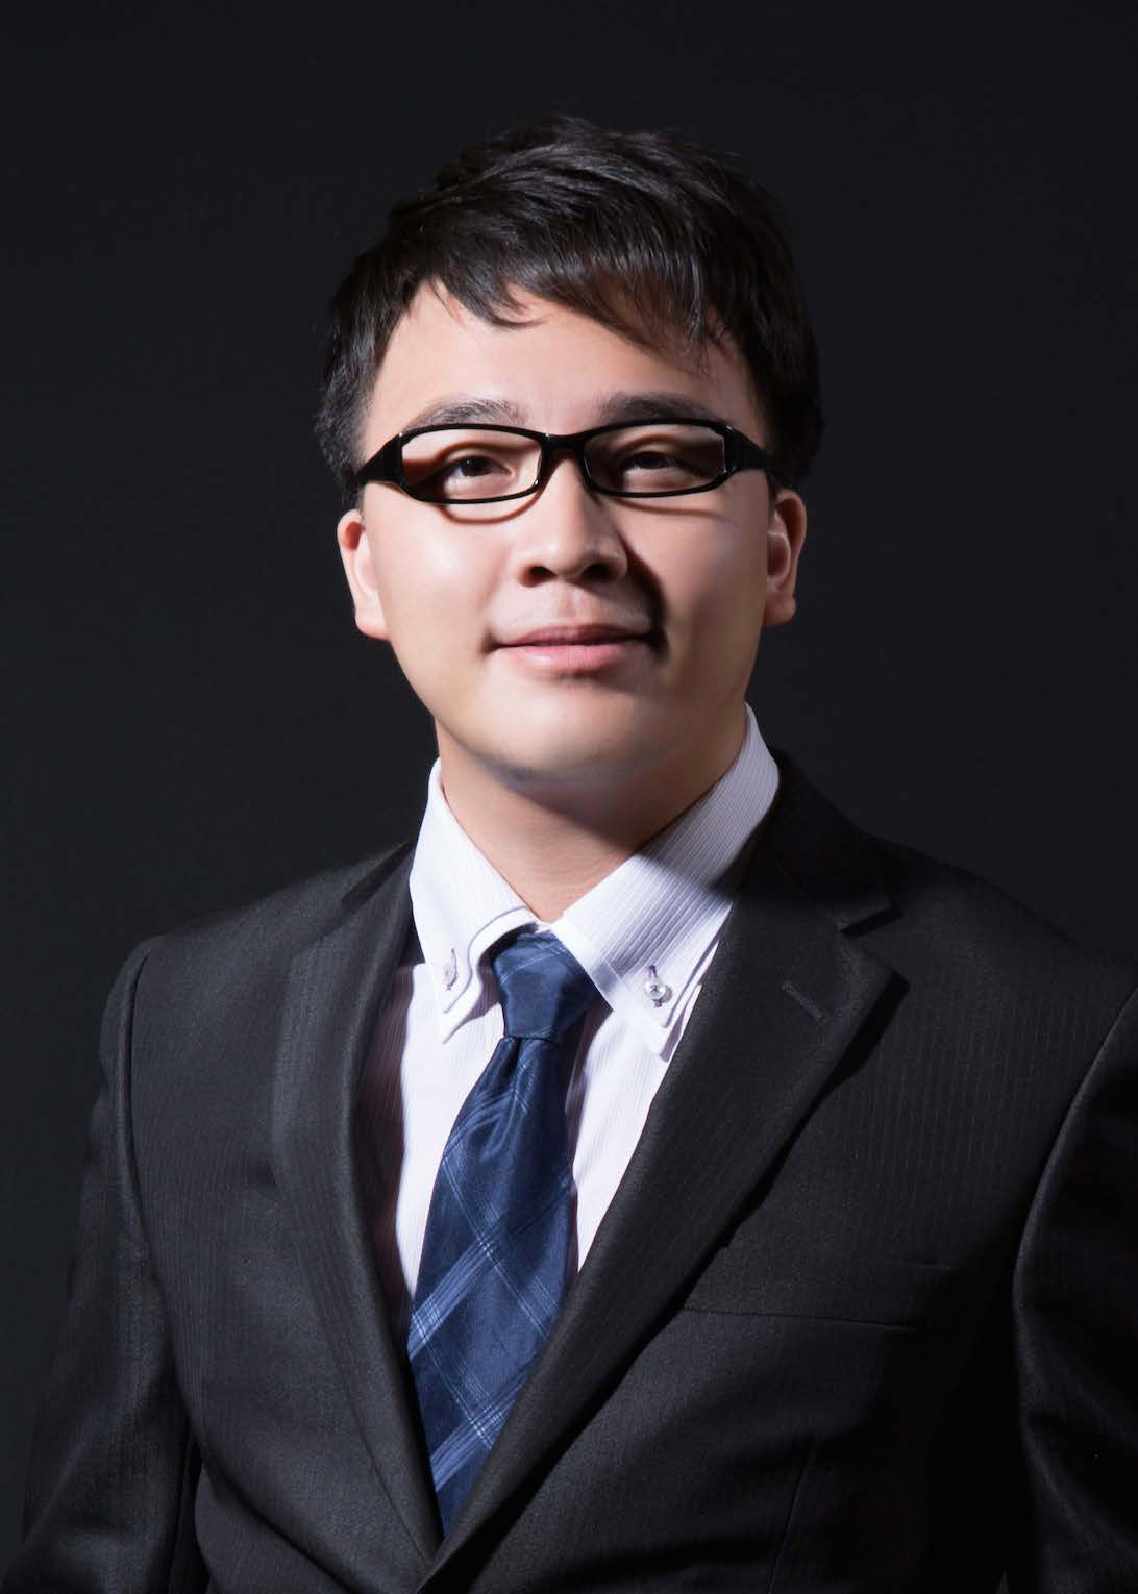
\includegraphics[width=1in,height=1.25in,clip,keepaspectratio]{Huang.pdf}}]
{Ming-Chun Huang} (M'14) is an assistant professor in the Electrical Engineering and Computer Science Department at Case Western Reserve
University~\cite{Sailab}. He has a PhD in computer science from the University of California, Los Angeles (UCLA). Dr. Huang has multiple years
experiences in pressure sensitive medical devices development, pressure map analysis, and physiological signal extraction research.
He is an expert in mHealth, telemedicine, and non-invasive sensing system design. His board research interests includes the area of
wearable computing, health informatics, big data analysis, human computer interaction, sensor, network, augmented reality, and
applications of Internet of Things. He received the Best Medical and Performance Application Paper Award from the IEEE Conference on
Implantable and Wearable Body Sensor Networks in $2013$ and the Best Demonstration Award in ACM Wireless Health Conference in $2011$.
\end{IEEEbiography} 